\documentclass{article}
%\usepackage{tex4ht}
\usepackage{amsmath}
\usepackage{amsfonts}
\usepackage{amssymb}
\usepackage{amsthm}
\usepackage{graphicx}
\usepackage{color}
\usepackage{float}
\usepackage{dsfont}
\usepackage{diagbox}
\setlength{\parskip}{0.5\baselineskip}
\author{Zhuo Liu (0983311)}
\title{Project on Automatic Learning (Phase 3)}
\date{March 18, 2014}

\definecolor{lightgray}{gray}{0.5}


\begin{document}
\maketitle


\section{Introduction}

In this report, we will apply supported vector machine (SVM) to build classifiers on the large and small data sets, and test their performances. Since both data sets are of multiple classes, we will use ``1-vs-1'' approach to build the classifiers, i.e., suppose there are $k$ classes, we need to use SVM to build $\frac{k(k-1)}{2}$ binary separators, and using vote strategy to classify a new observation. The performance of a classifier is then evaluated by number of supported vectors that appear in any $\frac{k(k-1)}{2}$ separators, mean and standard deviation of 10 accuracies by using 10-fold cross validation. Here, accuracies are over all the classes, not only two classes. In this report, we will try three different kernels for SVM: linear, polynomial and Gaussian, i.e.
\begin{align}
 & Linear\ kernel:\ k(x,y) = <x,y>_{\mathbb{R}^{p}} \\
 & Polynomial\ kernel:\ k(x,y) = (1+<x,y>_{\mathbb{R}^{p}})^{r} \\
 & Gaussian\ kernel:\ k(x,y) = exp(-\frac{||x-y||^{2}}{2\sigma^{2}})
\end{align}
In short, SVM is to find the separator with the form:
\begin{equation}
 g(x) = <u,x> + b
\end{equation}
where $<,>$ can be the regular inner product in $\mathbb{R}^{p}$ or the inner product in a Hilbert space defined by kernel function. $u$, $b$ satisfy the minimization problem:
\begin{equation}
 \min\{\frac{1}{2}||u||^{2} + c\sum \xi_{i}\}
\end{equation}
with constraints
\begin{align}
 \begin{cases}
  \xi_{i} \geq 0 \\
  \xi_{i}-(1-y_{i}g(x_{i})) \geq 0
 \end{cases}
\end{align}
Therefore, besides choosing proper parameters in kernel function, we need also to choose optimal parameters $c$ in (5). After determining the optimal parameters for each classifiers, we will draw the graph of observations where all the supported vectors are marked, and show the numbers of supported vectors, means and standard deviations of all $\frac{k(k-1)}{2}$ separators, and give the histograms of non-zero $\alpha_{i}$ in the best and worst separators among those $\frac{k(k-1)}{2}$ separators.

In phase 2, we have already build linear classifier and non-linear classifier on principle components space and kernel principle components space (for both polynomial kernel and Gaussian kernel), so we can also compare those results to the result obtained by SVM.

%%% ------------------------------------------------------------------------------
\goodbreak

\section{Database: the Large One}

We test each classifiers by 10-fold cross validation, i.e., randomly and equally sepearate data set into 10 subsets, choose 1 as test set, and union of the rest 9 to be training set, then build classifier based on training set and get the accuracy on the test set. We can do this 10 times, and the mean of 10 accuracies will be used to determining the optimal parameters.

\subsection{Linear Kernel}

The total number of observations in the data set is 1593. The following table shows the accuracies and the number of supported vectors for different choices of $c$ in (5):  

\scalebox{0.67}{
 \begin{tabular}{|c|c|c|c|c|c|c|c|}
  \hline
  c                   & 0.001         & 0.003         & 0.005         & 0.008         & 0.01          & 0.1           & 1             \\ \hline
  Accuracy            & $92.40427 \%$ & $93.65976 \%$ & $94.09918 \%$ & $94.09918 \%$ & $94.03641 \%$ & $93.59699 \%$ & $93.59699 \%$ \\ \hline
  Number of SVs       & 1218          & 1003          & 930           & 885           & 872           & 878           & 878           \\ \hline
 \end{tabular}
}
  
So $c=0.008$ is the optimal parameter. The following two tables shows the perfomance of the classifier by choosing $c=0.008$. (The first table contains the information about means and standard deviations of 10 accuracies by 10-fold cross validation. Since separator over class i and j is equivalent to separator over class j and i, so either means or standard deviations need only half of the 10 by 10 matrix. In order to save space, we combine these two information into one table, so the upper triangular part of the first table shows the means of accuracies, and lower triangular part shows the stand deviations. Similarly, the second table shows the number of supported vectors by using SVM over class i and class j. All the tables in the rest of the report showing these information has the same scheme.)

\scalebox{0.82}{
 \begin{tabular}{|c|c|c|c|c|c|c|c|c|c|c|}
  \hline
  class  & '0'       & '1'       & '2'       & '3'       & '4'       & '5'       & '6'       & '7'       & '8'       & '9'         \\ \hline
  '0'    & NA        & $99.69\%$ & $99.38\%$ & $100.0\%$ & $99.38\%$ & $99.38\%$ & $99.07\%$ & $99.69\%$ & $99.37\%$ & $99.06\%$ \\ \hline
  '1'    & $0.98821$ & NA        & $97.51\%$ & $98.44\%$ & $96.28\%$ & $99.38\%$ & $100.0\%$ & $98.13\%$ & $99.37\%$ & $97.19\%$ \\ \hline
  '2'    & $1.31762$ & $2.46503$ & NA        & $98.74\%$ & $98.13\%$ & $99.06\%$ & $99.38\%$ & $99.68\%$ & $98.41\%$ & $99.05\%$ \\ \hline
  '3'    & $0.00000$ & $2.20246$ & $1.64012$ & NA        & $100.0\%$ & $97.17\%$ & $100.0\%$ & $98.42\%$ & $98.73\%$ & $94.64\%$ \\ \hline
  '4'    & $1.31762$ & $3.48381$ & $2.18502$ & $0.00000$ & NA        & $99.69\%$ & $98.45\%$ & $97.18\%$ & $99.68\%$ & $98.74\%$ \\ \hline
  '5'    & $1.31762$ & $1.31767$ & $1.50952$ & $1.77615$ & $0.98821$ & NA        & $98.44\%$ & $99.37\%$ & $99.68\%$ & $99.37\%$ \\ \hline
  '6'    & $1.50952$ & $0.00000$ & $1.31762$ & $0.00000$ & $1.62742$ & $2.20971$ & NA        & $99.37\%$ & $99.37\%$ & $100.0\%$ \\ \hline
  '7'    & $0.98821$ & $2.18502$ & $0.98821$ & $2.21784$ & $2.30757$ & $1.33908$ & $1.33908$ & NA        & $98.40\%$ & $97.78\%$ \\ \hline
  '8'    & $1.31762$ & $1.33908$ & $2.27328$ & $1.65304$ & $0.98821$ & $1.02009$ & $1.36012$ & $1.67930$ & NA        & $96.81\%$ \\ \hline
  '9'    & $1.50952$ & $3.10759$ & $1.52600$ & $4.46340$ & $2.19484$ & $1.31762$ & $0.00000$ & $2.61277$ & $3.01814$ & NA        \\ \hline
 \end{tabular}
}

\scalebox{0.82}{
 \begin{tabular}{|c|c|c|c|c|c|c|c|c|c|c|}
  \hline
  class& '0'& '1'& '2'& '3'& '4'& '5'& '6'& '7'& '8'& '9'\\ \hline
  '0'  & NA & 47 & 41 & 52 & 71 & 68 & 81 & 47 & 63 & 48 \\ \hline
  '1'  & NA & NA & 75 & 66 & 111& 50 & 63 & 88 & 98 & 68 \\ \hline
  '2'  & NA & NA & NA & 65 & 55 & 64 & 59 & 59 & 89 & 71 \\ \hline
  '3'  & NA & NA & NA & NA & 53 & 119& 61 & 83 & 105& 89 \\ \hline
  '4'  & NA & NA & NA & NA & NA & 58 & 90 & 69 & 49 & 57 \\ \hline
  '5'  & NA & NA & NA & NA & NA & NA & 93 & 87 & 90 & 81 \\ \hline
  '6'  & NA & NA & NA & NA & NA & NA & NA & 70 & 98 & 47 \\ \hline
  '7'  & NA & NA & NA & NA & NA & NA & NA & NA & 91 & 67 \\ \hline
  '8'  & NA & NA & NA & NA & NA & NA & NA & NA & NA & 82 \\ \hline
  '9'  & NA & NA & NA & NA & NA & NA & NA & NA & NA & NA \\ \hline
 \end{tabular}
}

Figure 1 shows the observations in PC space when choosing optimal parameter $c=0.008$ (all the supported vectors are marked by ``cross'' sign).

\begin{figure}[htp]
\centering
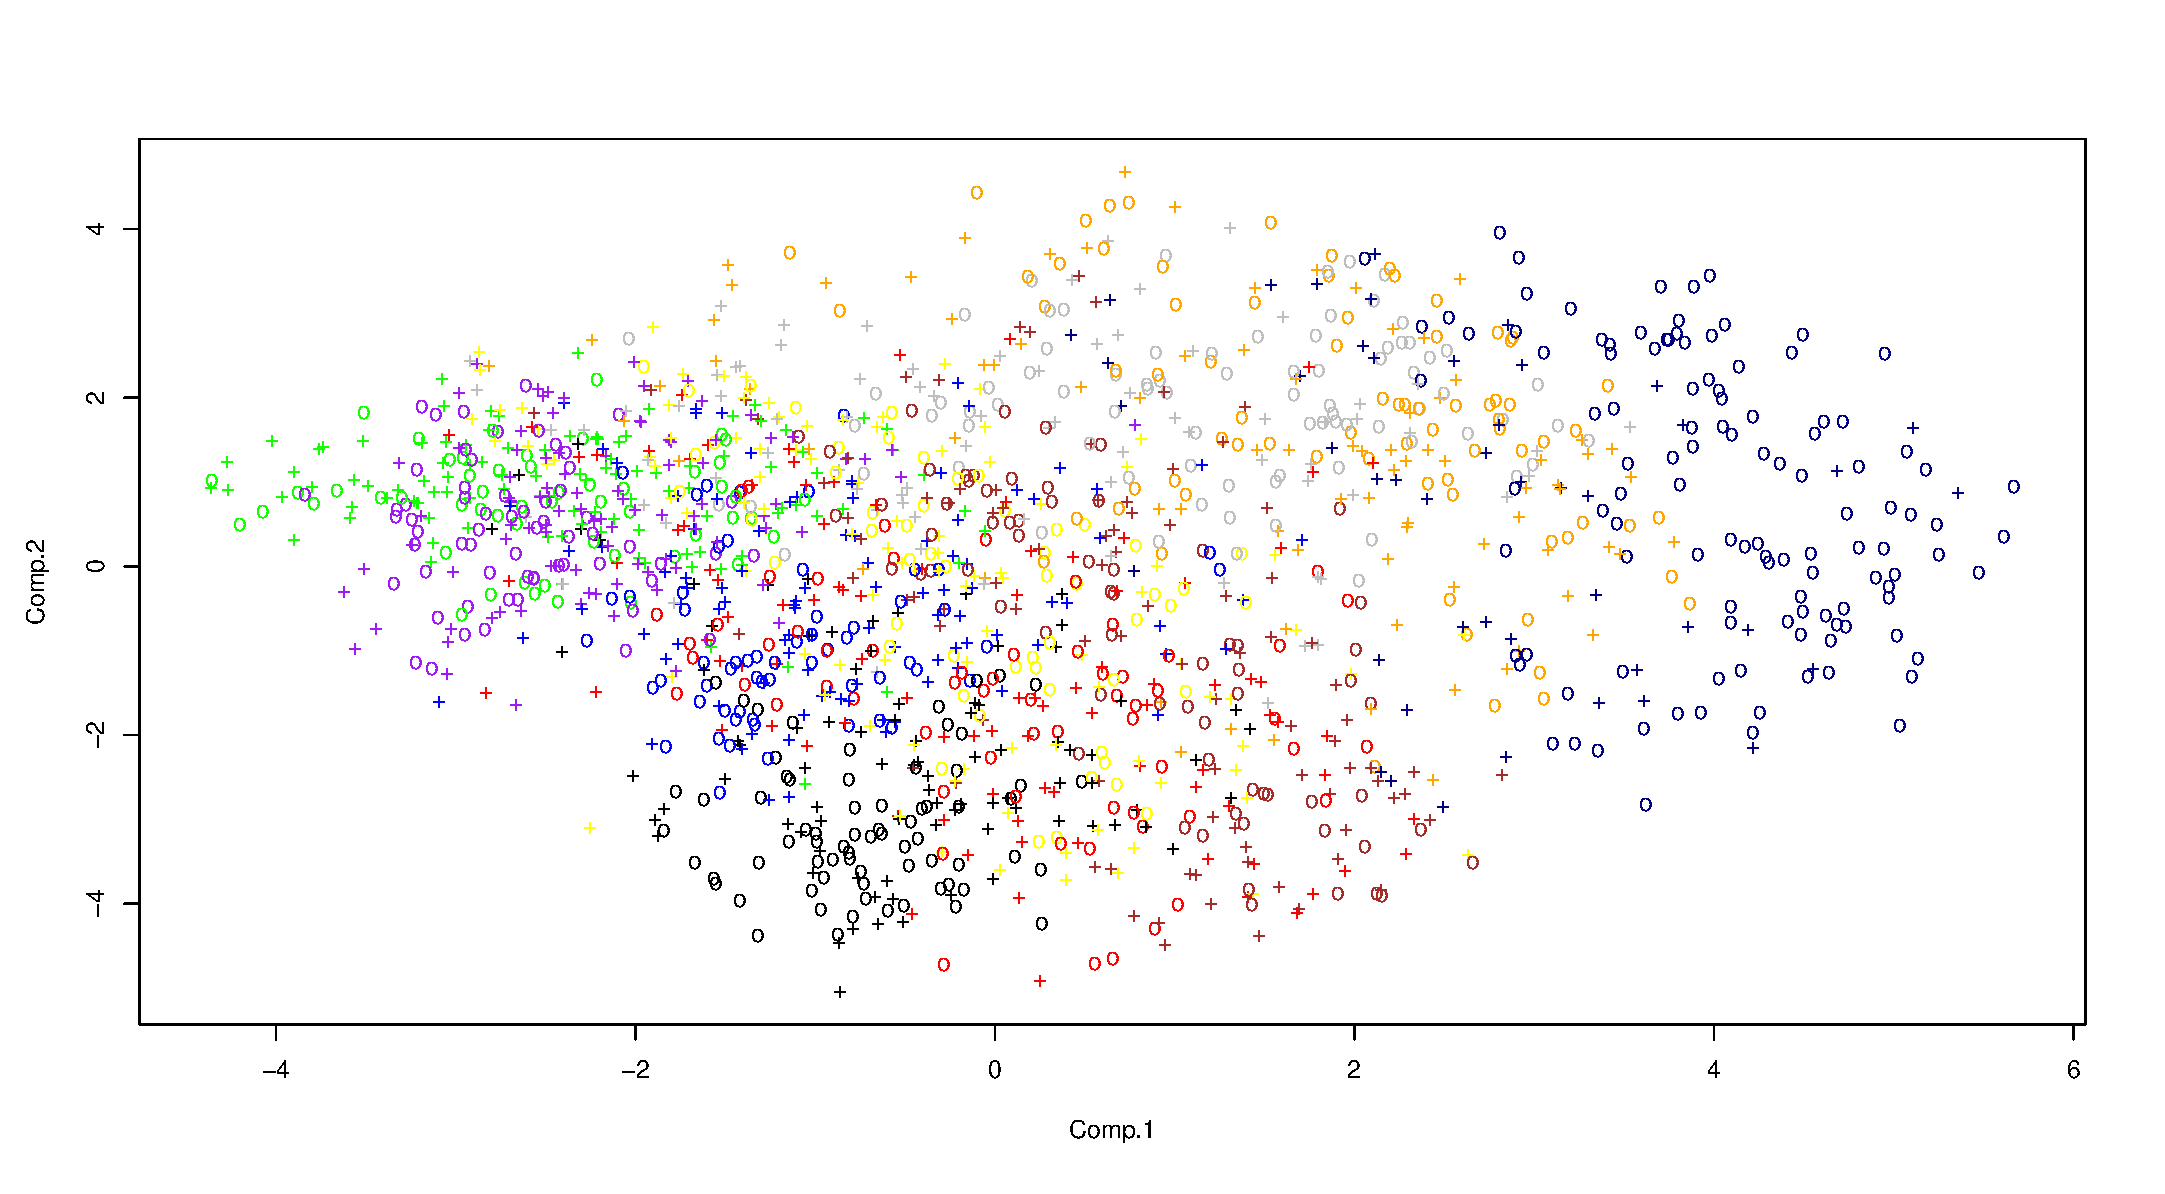
\includegraphics[width=12.1cm]{large_svm_linear.eps}
\caption{\textit{Projection of data into first two PC space. Here, ``cross'' represent the supported vector by using linear kernel, and the colors represent different classes: navy--0, green--1, blue--2, black--3, grey--4, brown--5, orange--6, purple--7, yellow--8, red--9.}}
\end{figure}

Among the 45 SVM separators, separator over class '6' and class '9' has best perfomance, and separator over class '3' and class '9' has worst performance. Figure 2 show the histograms of non-zero $\alpha_{i}$ of these two separators.

\begin{figure}[htp]
\centering
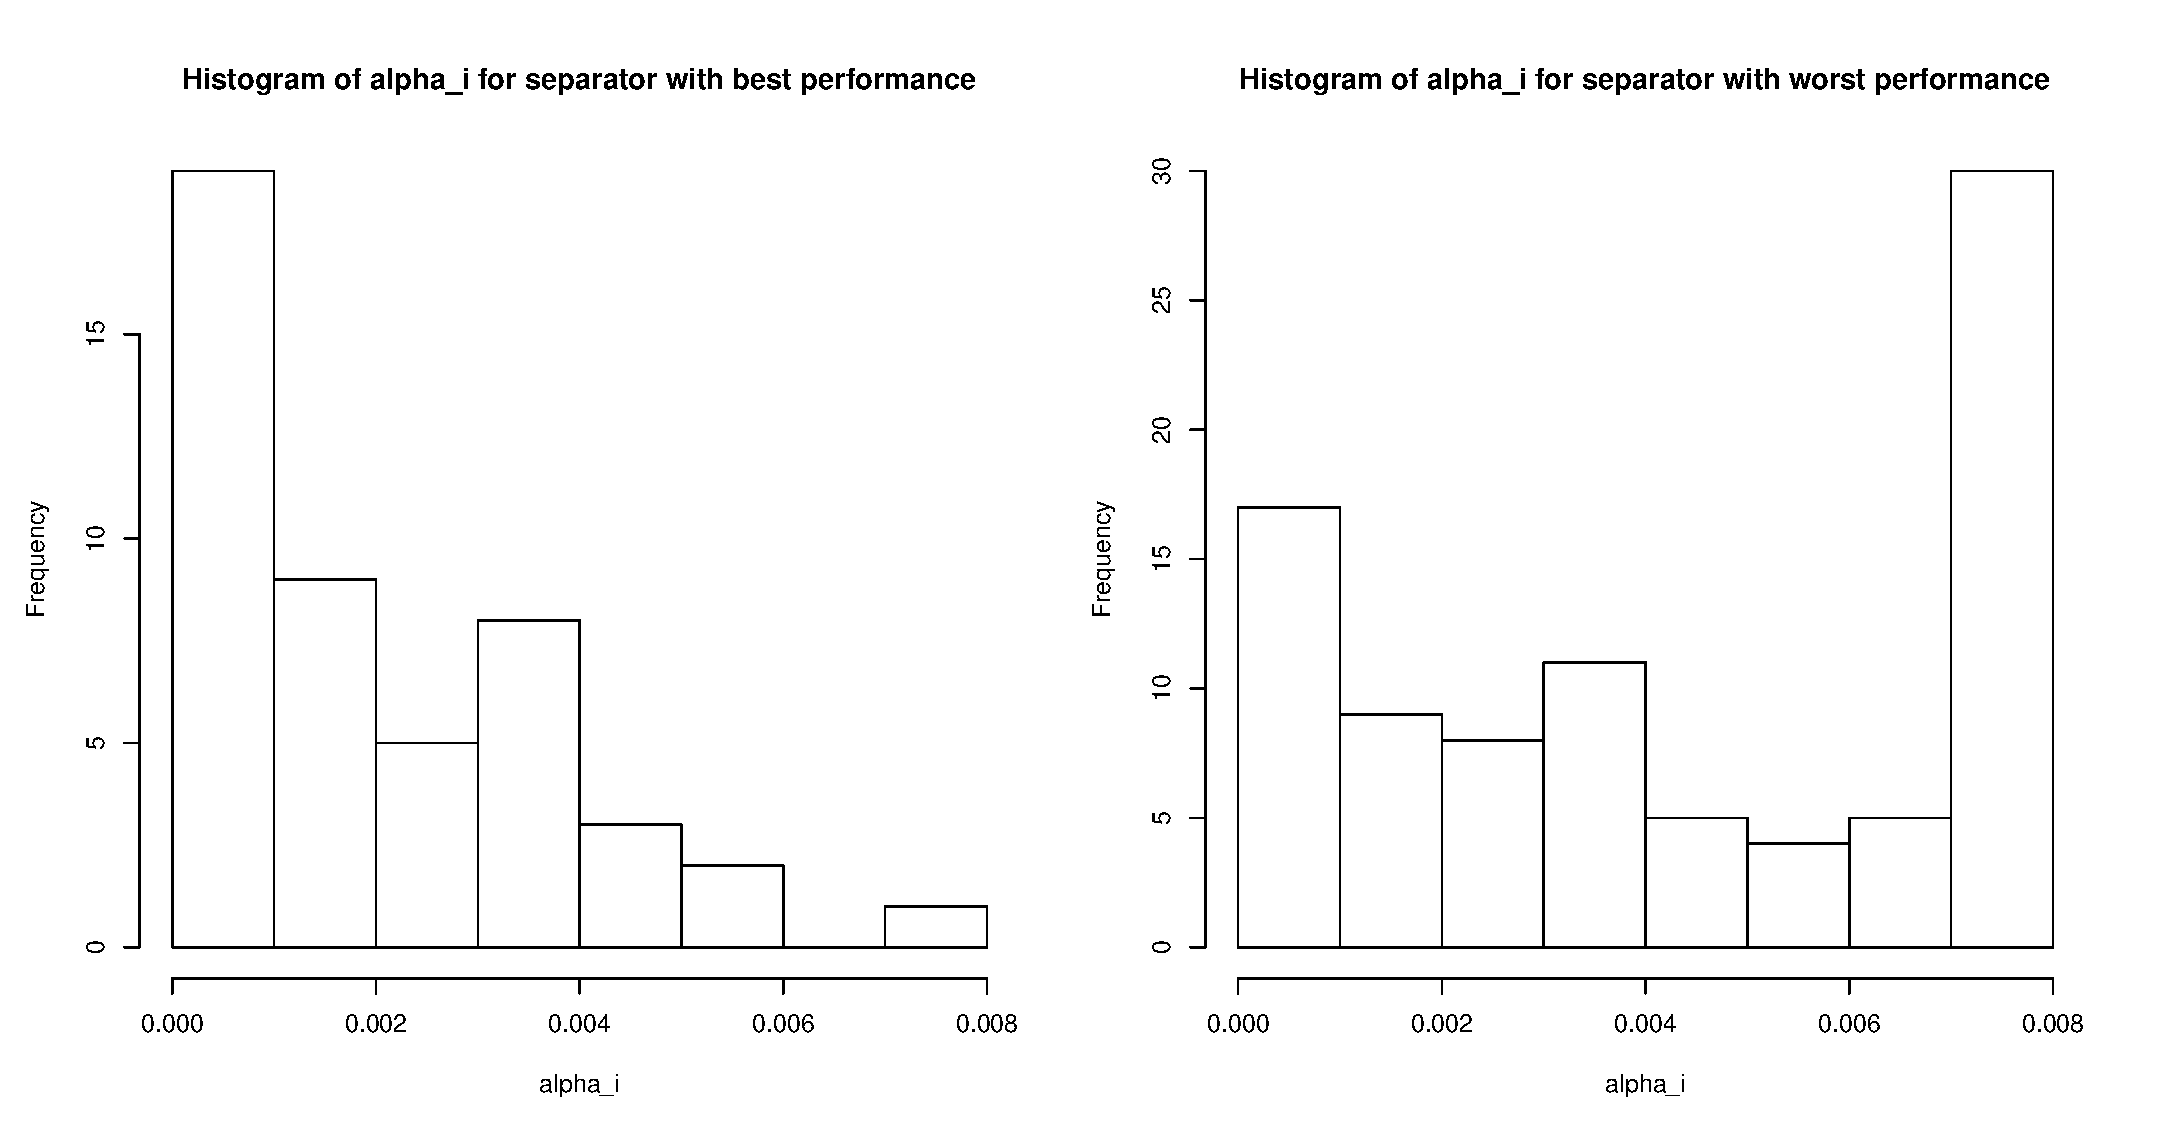
\includegraphics[width=12.1cm]{large_hist_linear.eps}
\caption{\textit{Histograms of $\alpha_{i}$ for SVM separators with best and worst performances by using linear kernel on large data set with optimal parameter. Left: best, separator over class '6' and class '9', $\#$ of SVs is 47. Right: worst, separator over class '3' and '9', $\#$ of SVs is 89.}}
\end{figure}

%%% ------------------------------------------------------------------------------
\goodbreak

\subsection{Polynomial Kernel}

The following table shows the accuracies by choosing different $c$ in (5) and $r$ in (2):

\scalebox{0.85}{
 \begin{tabular}{|c|c|c|c|c|c|c|}
  \hline
  \diagbox{r}{c} & $10^{-5}$ & $2\times10^{-5}$ & $3\times10^{-5}$ & $4\times10^{-5}$ & $5\times10^{-5}$ & $10^{-4}$ \\ \hline
  2              & $95.16635 \%$ & $95.79410 \%$ & $95.79410 \%$ & $95.73123 \%$ & $95.73123 \%$ & $95.73123 \%$ \\ \hline
  3              & $95.35468 \%$ & $95.35468 \%$ & $95.35468 \%$ & $95.35468 \%$ & $95.35468 \%$ & $95.35468 \%$ \\ \hline
  4              & $88.57502 \%$ & $88.57502 \%$ & $88.57502 \%$ & $88.57502 \%$ & $88.57502 \%$ & $88.57502 \%$ \\ \hline
  5              & $70.80979 \%$ & $70.80979 \%$ & $70.80979 \%$ & $70.80979 \%$ & $70.80979 \%$ & $70.80979 \%$ \\ \hline
 \end{tabular}
}

Next table shows the number of supported vectors for different $c$ and $r$:

\scalebox{1}{
 \begin{tabular}{|c|c|c|c|c|c|c|}
  \hline
  \diagbox{r}{c} & $10^{-5}$ & $2\times10^{-5}$ & $3\times10^{-5}$ & $4\times10^{-5}$ & $5\times10^{-5}$ & $10^{-4}$ \\ \hline
  2              & 1304 & 1303 & 1306 & 1306 & 1306 & 1306 \\ \hline
  3              & 1382 & 1382 & 1382 & 1382 & 1382 & 1382 \\ \hline
  4              & 1477 & 1477 & 1477 & 1477 & 1477 & 1477 \\ \hline
  5              & 1526 & 1526 & 1526 & 1526 & 1526 & 1526 \\ \hline
 \end{tabular}
}

Therefore, we choose $c=2\times10^{-5}$ and $r=2$ as our optimal parameters. The following two tables shows the perfomance of the classifier by choosing optimal parameters. 
Figure 3 shows the supported vectors among all vectors. We can observe from these two tables that among the 45 SVM separators, separator over class '3' and class '6' has best perfomance, and separator over class '5' and class '9' has worst performance. Figure 4 shows the histogram of non-zero $\alpha_{i}$ for these two separators. 

\scalebox{0.82}{
 \begin{tabular}{|c|c|c|c|c|c|c|c|c|c|c|}
  \hline
  class& '0'       & '1'       & '2'       & '3'       & '4'       & '5'       & '6'       & '7'       & '8'       & '9'       \\ \hline
  '0'  & NA        & $99.38\%$ & $99.75\%$ & $99.69\%$ & $98.14\%$ & $98.13\%$ & $98.76\%$ & $99.37\%$ & $99.37\%$ & $97.81\%$ \\ \hline
  '1'  & $1.31762$ & NA        & $97.51\%$ & $99.38\%$ & $94.12\%$ & $99.69\%$ & $99.38\%$ & $97.81\%$ & $97.48\%$ & $97.81\%$ \\ \hline
  '2'  & $2.18502$ & $3.84148$ & NA        & $98.11\%$ & $98.13\%$ & $99.69\%$ & $100.0\%$ & $97.48\%$ & $95.86\%$ & $98.42\%$ \\ \hline
  '3'  & $0.98821$ & $1.31762$ & $2.67826$ & NA        & $99.38\%$ & $97.48\%$ & $100.0\%$ & $96.85\%$ & $97.13\%$ & $93.06\%$ \\ \hline
  '4'  & $3.01904$ & $4.48198$ & $2.63523$ & $1.31762$ & NA        & $99.69\%$ & $97.20\%$ & $98.12\%$ & $99.05\%$ & $97.81\%$ \\ \hline
  '5'  & $2.18502$ & $0.98821$ & $0.98821$ & $2.50261$ & $0.98821$ & NA        & $99.06\%$ & $99.05\%$ & $98.09\%$ & $90.22\%$ \\ \hline
  '6'  & $2.18502$ & $1.29784$ & $0.00000$ & $0.00000$ & $2.73520$ & $1.50952$ & NA        & $99.37\%$ & $99.68\%$ & $98.43\%$ \\ \hline
  '7'  & $1.97642$ & $4.17967$ & $3.22981$ & $2.55191$ & $1.62271$ & $1.52600$ & $1.31762$ & NA        & $97.76\%$ & $98.10\%$ \\ \hline
  '8'  & $1.31762$ & $4.11608$ & $3.00827$ & $2.37615$ & $1.52600$ & $2.24305$ & $1.02009$ & $2.62088$ & NA        & $91.37\%$ \\ \hline
  '9'  & $2.10921$ & $3.31047$ & $1.66868$ & $4.12560$ & $2.57273$ & $6.34766$ & $1.64702$ & $2.19821$ & $5.07747$ & NA        \\ \hline
 \end{tabular}
}

\scalebox{0.82}{
 \begin{tabular}{|c|c|c|c|c|c|c|c|c|c|c|}
  \hline
  class& '0'& '1' & '2' & '3' & '4' & '5' & '6' & '7' & '8' & '9' \\ \hline
  '0'  & NA & 118 & 241 & 119 & 149 & 151 & 151 & 129 & 133 & 255 \\ \hline
  '1'  & NA & NA  & 249 & 256 & 231 & 243 & 150 & 258 & 177 & 246 \\ \hline
  '2'  & NA & NA  & NA  & 288 & 257 & 254 & 236 & 284 & 269 & 273 \\ \hline
  '3'  & NA & NA  & NA  & NA  & 265 & 229 & 146 & 186 & 189 & 290 \\ \hline
  '4'  & NA & NA  & NA  & NA  & NA  & 261 & 192 & 269 & 262 & 274 \\ \hline
  '5'  & NA & NA  & NA  & NA  & NA  & NA  & 193 & 204 & 192 & 294 \\ \hline
  '6'  & NA & NA  & NA  & NA  & NA  & NA  & NA  & 158 & 179 & 269 \\ \hline
  '7'  & NA & NA  & NA  & NA  & NA  & NA  & NA  & NA  & 179 & 271 \\ \hline
  '8'  & NA & NA  & NA  & NA  & NA  & NA  & NA  & NA  & NA  & 296 \\ \hline
  '9'  & NA & NA  & NA  & NA  & NA  & NA  & NA  & NA  & NA  & NA  \\ \hline
 \end{tabular}
}

\begin{figure}[htp]
\centering
\includegraphics[width=12.1cm]{large_svm_polynomial.eps}
\caption{\textit{Projection of data into first two PC space. Here, ``cross'' represent the supported vector by using polynomial kernel, and the colors represent different classes: navy--0, green--1, blue--2, black--3, grey--4, brown--5, orange--6, purple--7, yellow--8, red--9.}}
\end{figure}

\begin{figure}[htp]
\centering
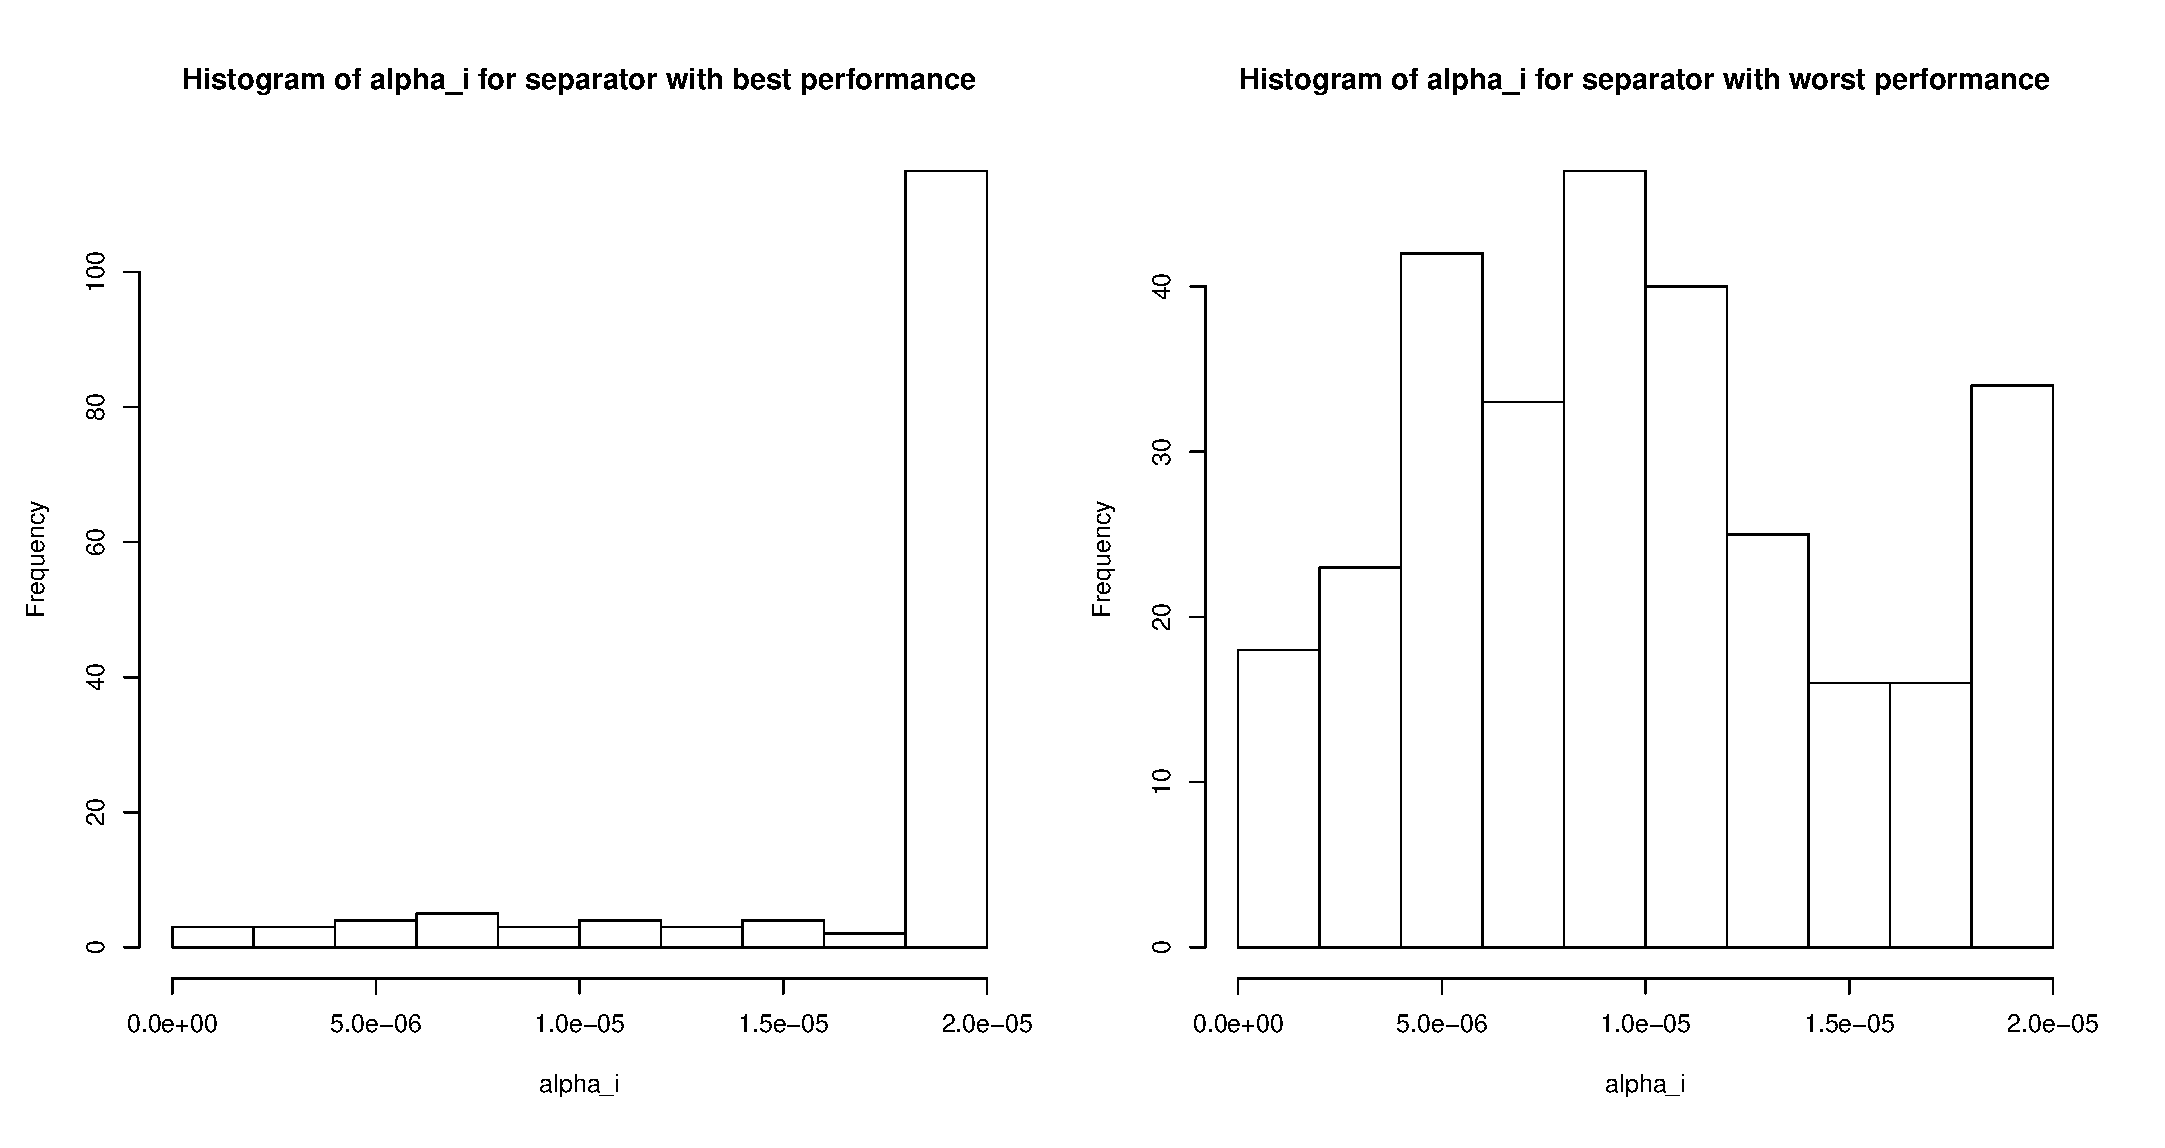
\includegraphics[width=12.1cm]{large_hist_polynomial.eps}
\caption{\textit{Histograms of $\alpha_{i}$ for SVM separators with best and worst performances by using polynomial kernel on large data set with optimal parameter. Left: best, separator over class '3' and class '6', $\#$ of SVs is 146. Right: worst, separator over class '5' and '9', $\#$ of SVs is 294.}}
\end{figure}

%%% ------------------------------------------------------------------------------
\goodbreak

\subsection{Gaussian Kernel}

At last, we will see the SVM by using Gaussian kernel. The parameters are $c$ and $\sigma$, but instead of $\sigma$, we will use $\sigma^{*} = \frac{1}{2\sigma^{2}}$ in the following accuracy table:

\scalebox{0.71}{
 \begin{tabular}{|c|c|c|c|c|c|c|c|}
  \hline
  \diagbox{$\sigma^{*}$}{c} & 0.2         & 0.5           & 1             & 10            & 20            & 50            & 100           \\ \hline
  0.0001                  & $12.24105 \%$ & $71.12367 \%$ & $85.05964 \%$ & $93.40866 \%$ & $93.97363 \%$ & $94.28751 \%$ & $93.72254 \%$ \\ \hline
  0.001                   & $88.44947 \%$ & $92.71814 \%$ & $93.78531 \%$ & $95.22913 \%$ & $95.22913 \%$ & $95.22913 \%$ & $95.22913 \%$ \\ \hline
  0.003                   & $91.21155 \%$ & $94.28751 \%$ & $95.16635 \%$ & $95.79410 \%$ & $95.79410 \%$ & $95.79410 \%$ & $95.79410 \%$ \\ \hline
  0.005                   & $90.83490 \%$ & $94.22473 \%$ & $95.54300 \%$ & $95.66855 \%$ & $95.66855 \%$ & $95.66855 \%$ & $95.66855 \%$ \\ \hline
  0.007                   & $88.32392 \%$ & $93.78531 \%$ & $95.41745 \%$ & $95.60578 \%$ & $95.60578 \%$ & $95.60578 \%$ & $95.60578 \%$ \\ \hline
  0.01                    & $64.53233 \%$ & $91.71375 \%$ & $94.03641 \%$ & $94.03641 \%$ & $94.03641 \%$ & $94.03641 \%$ & $94.03641 \%$ \\ \hline
  0.1                     & $6.465788 \%$ & $6.465788 \%$ & $6.654112 \%$ & $6.779661 \%$ & $6.779661 \%$ & $6.779661 \%$ & $6.779661 \%$ \\ \hline
 \end{tabular}
}

The following table shows the number of SVs by different $\sigma^{*}$ and $c$:

\scalebox{1}{
 \begin{tabular}{|c|c|c|c|c|c|c|c|}
  \hline
  \diagbox{$\sigma^{*}$}{c}& 0.2 & 0.5  & 1    & 10   & 20   & 50   & 100  \\ \hline
  0.0001                  & 1593 & 1586 & 1537 & 1089 & 976  & 883  & 886  \\ \hline
  0.001                   & 1486 & 1307 & 1173 & 1030 & 1031 & 1031 & 1031 \\ \hline
  0.003                   & 1420 & 1281 & 1225 & 1224 & 1224 & 1224 & 1224 \\ \hline
  0.005                   & 1454 & 1361 & 1347 & 1355 & 1355 & 1355 & 1355 \\ \hline
  0.007                   & 1516 & 1443 & 1444 & 1446 & 1446 & 1446 & 1446 \\ \hline
  0.01                    & 1572 & 1523 & 1521 & 1520 & 1520 & 1520 & 1520 \\ \hline
  0.1                     & 1593 & 1593 & 1593 & 1593 & 1593 & 1593 & 1593 \\ \hline
 \end{tabular}
}

Therefore, we choose $\sigma^{*}=0.003$ and $c=10$ as our optimal parameters. The following two tables shows the perfomance of the classifier by choosing optimal parameters. 
Figure 5 shows the supported vectors among all vectors. We can observe from these two tables that among the 45 SVM separators, separator over class '0' and class '3' has best perfomance, and separator over class '3' and class '9' has worst performance. Figure 6 shows the histograms of non-zero $\alpha_{i}$ of these two separators.

\scalebox{0.82}{
 \begin{tabular}{|c|c|c|c|c|c|c|c|c|c|c|}
  \hline
  class& '0'       & '1'       & '2'       & '3'       & '4'       & '5'       & '6'       & '7'       & '8'       & '9'       \\ \hline
  '0'  & NA        & $99.69\%$ & $99.28\%$ & $100.0\%$ & $99.38\%$ & $99.38\%$ & $99.07\%$ & $99.69\%$ & $99.37\%$ & $98.75\%$ \\ \hline
  '1'  & $0.98821$ & NA        & $99.07\%$ & $99.07\%$ & $97.52\%$ & $99.69\%$ & $100.0\%$ & $97.50\%$ & $99.37\%$ & $98.13\%$ \\ \hline
  '2'  & $1.31762$ & $1.50952$ & NA        & $99.06\%$ & $99.38\%$ & $99.69\%$ & $99.69\%$ & $100.0\%$ & $98.41\%$ & $99.68\%$ \\ \hline
  '3'  & $0.00000$ & $1.49449$ & $1.54223$ & NA        & $100.0\%$ & $96.86\%$ & $100.0\%$ & $98.74\%$ & $99.36\%$ & $96.53\%$ \\ \hline
  '4'  & $1.31762$ & $3.20350$ & $1.97642$ & $0.00000$ & NA        & $100.0\%$ & $99.38\%$ & $98.75\%$ & $100.0\%$ & $99.06\%$ \\ \hline
  '5'  & $1.31762$ & $0.98821$ & $0.98821$ & $3.31584$ & $0.00000$ & NA        & $98.44\%$ & $99.68\%$ & $99.68\%$ & $98.74\%$ \\ \hline
  '6'  & $1.50952$ & $0.00000$ & $0.98821$ & $0.00000$ & $1.31762$ & $2.20971$ & NA        & $99.37\%$ & $99.37\%$ & $100.0\%$ \\ \hline
  '7'  & $0.98821$ & $1.97642$ & $0.00000$ & $2.19484$ & $1.62702$ & $1.02009$ & $1.33908$ & NA        & $98.72\%$ & $98.42\%$ \\ \hline
  '8'  & $1.31762$ & $1.33908$ & $2.27328$ & $1.31762$ & $0.00000$ & $1.02009$ & $1.36012$ & $1.64012$ & NA        & $98.72\%$ \\ \hline
  '9'  & $1.62702$ & $2.18502$ & $0.98821$ & $3.10663$ & $1.52600$ & $1.62702$ & $0.00000$ & $2.26549$ & $1.65304$ & NA        \\ \hline
 \end{tabular}
}

\scalebox{0.82}{
 \begin{tabular}{|c|c|c|c|c|c|c|c|c|c|c|}
  \hline
  class& '0'& '1' & '2' & '3' & '4' & '5' & '6' & '7' & '8' & '9' \\ \hline
  '0'  & NA & 41  & 99  & 47  & 55  & 47  & 72  & 47  & 57  & 111 \\ \hline
  '1'  & NA & NA  & 153 & 149 & 89  & 129 & 60  & 176 & 73  & 135 \\ \hline
  '2'  & NA & NA  & NA  & 157 & 125 & 142 & 139 & 161 & 173 & 147 \\ \hline
  '3'  & NA & NA  & NA  & NA  & 118 & 85  & 50  & 68  & 82  & 170 \\ \hline
  '4'  & NA & NA  & NA  & NA  & NA  & 125 & 69  & 144 & 120 & 121 \\ \hline
  '5'  & NA & NA  & NA  & NA  & NA  & NA  & 70  & 72  & 73  & 173 \\ \hline
  '6'  & NA & NA  & NA  & NA  & NA  & NA  & NA  & 63  & 76  & 117 \\ \hline
  '7'  & NA & NA  & NA  & NA  & NA  & NA  & NA  & NA  & 74  & 129 \\ \hline
  '8'  & NA & NA  & NA  & NA  & NA  & NA  & NA  & NA  & NA  & 185 \\ \hline
  '9'  & NA & NA  & NA  & NA  & NA  & NA  & NA  & NA  & NA  & NA  \\ \hline
 \end{tabular}
}

\begin{figure}[htp]
\centering
\includegraphics[width=12.1cm]{large_svm_gaussian.eps}
\caption{\textit{Projection of data into first two PC space. Here, ``cross'' represent the supported vector by using Gaussian kernel, and the colors represent different classes: navy--0, green--1, blue--2, black--3, grey--4, brown--5, orange--6, purple--7, yellow--8, red--9.}}
\end{figure}

\begin{figure}[htp]
\centering
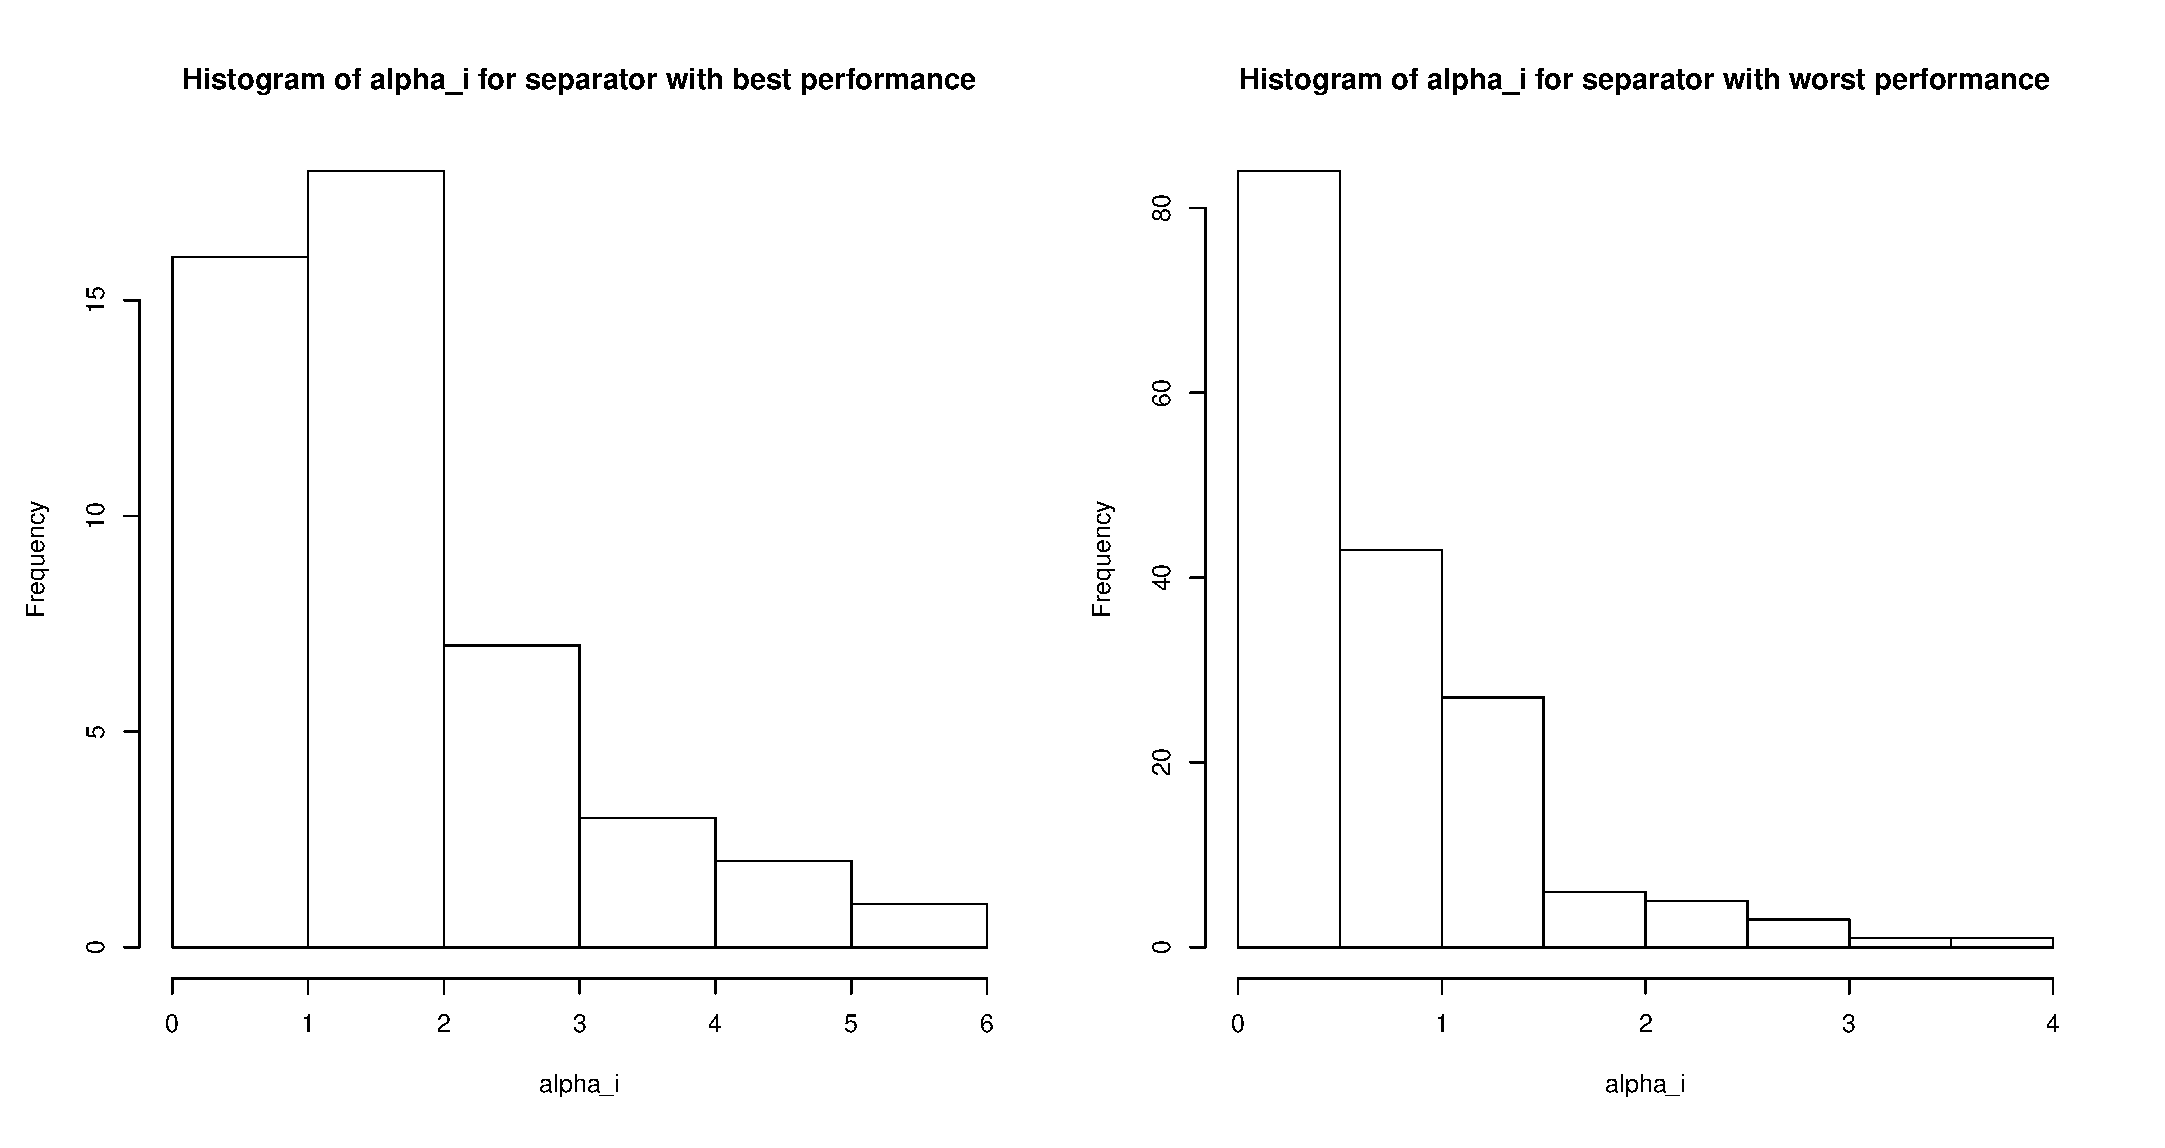
\includegraphics[width=12.1cm]{large_hist_gaussian.eps}
\caption{\textit{Histograms of $\alpha_{i}$ for SVM separators with best and worst performances by using Gaussian kernel on large data set with optimal parameter. Left: best, separator over class '0' and class '3', $\#$ of SVs is 47. Right: worst, separator over class '3' and '9', $\#$ of SVs is 170.}}
\end{figure}

%%% ------------------------------------------------------------------------------
\goodbreak

\newpage

\section{Database: the Small One}

\subsection{Linear Kernel}

By different experiments, we choose $c=10$ as our optimal parameter, the following table shows the accuracies for different choices of $c$:  

\scalebox{0.75}{
 \begin{tabular}{|c|c|c|c|c|c|c|}
  \hline
  c                   & 0.5           & 1             & 5             & 10            & 20            & 50            \\ \hline
  Accuracy            & $94.67532 \%$ & $95.28139 \%$ & $95.84416 \%$ & $96.01732 \%$ & $95.88745 \%$ & $95.84416 \%$ \\ \hline
  Number of SVs       & 509           & 457           & 386           & 361           & 344           & 332           \\ \hline
 \end{tabular}
}
  
We choose $c=10$ as optimal parameter. The following two tables shows the perfomance of the classifier by choosing optimal parameters. Figure 7 shows the supported vectors among all vectors. We can observe from these two tables that among the 21 SVM separators, separator over class 'foliage' and class 'sky' has best perfomance, and separator over class 'foliage' and class 'window' has worst performance. Figure 8 shows the histograms of non-zero $\alpha_{i}$ for these two separators.

\scalebox{0.82}{
 \begin{tabular}{|c|c|c|c|c|c|c|c|}
  \hline
  class     & brickface & cement    & foliage   & grass     & path      & sky       & window    \\ \hline
  brickface & NA        & $99.55\%$ & $99.70\%$ & $100.0\%$ & $100.0\%$ & $100.0\%$ & $99.09\%$ \\ \hline
  cement    & $1.43740$ & NA        & $98.18\%$ & $99.84\%$ & $100.0\%$ & $100.0\%$ & $94.55\%$ \\ \hline
  foliage   & $0.63884$ & $1.56484$ & NA        & $99.70\%$ & $100.0\%$ & $100.0\%$ & $91.21\%$ \\ \hline
  grass     & $0.00000$ & $0.47913$ & $0.63884$ & NA        & $99.70\%$ & $100.0\%$ & $99.85\%$ \\ \hline
  path      & $0.00000$ & $0.00000$ & $0.00000$ & $0.63884$ & NA        & $100.0\%$ & $100.0\%$ \\ \hline
  sky       & $0.00000$ & $0.00000$ & $0.00000$ & $0.00000$ & $0.00000$ & NA        & $100.0\%$ \\ \hline
  window    & $1.05940$ & $2.69150$ & $4.21347$ & $0.47913$ & $0.00000$ & $0.00000$ & NA        \\ \hline
 \end{tabular}
}

\scalebox{0.82}{
 \begin{tabular}{|c|c|c|c|c|c|c|c|}
  \hline
  class     & brickface & cement    & foliage   & grass     & path      & sky       & window    \\ \hline
  brickface  & NA & 14 & 14 & 10 & 8  & 9  & 17 \\ \hline
  cement  & NA & NA & 29 & 11 & 14 & 9  & 78 \\ \hline
  foliage  & NA & NA & NA & 10 & 10 & 6  & 163 \\ \hline
  grass  & NA & NA & NA & NA & 10 & 11 & 8  \\ \hline
  path  & NA & NA & NA & NA & NA & 7  & 11 \\ \hline
  sky  & NA & NA & NA & NA & NA & NA & 8  \\ \hline
  window  & NA & NA & NA & NA & NA & NA & NA \\ \hline
 \end{tabular}
}

\begin{figure}[htp]
\centering
\includegraphics[width=12.1cm]{small_svm_linear.eps}
\caption{\textit{Projection of data into first two PC space. Here, ``cross'' represent the supported vector by using linear kernel, and the colors represent different classes: red--brickface, brown--sky, blue--foliage, green--cement, orange--window, grey--path, black--grass.}}
\end{figure}

\begin{figure}[htp]
\centering
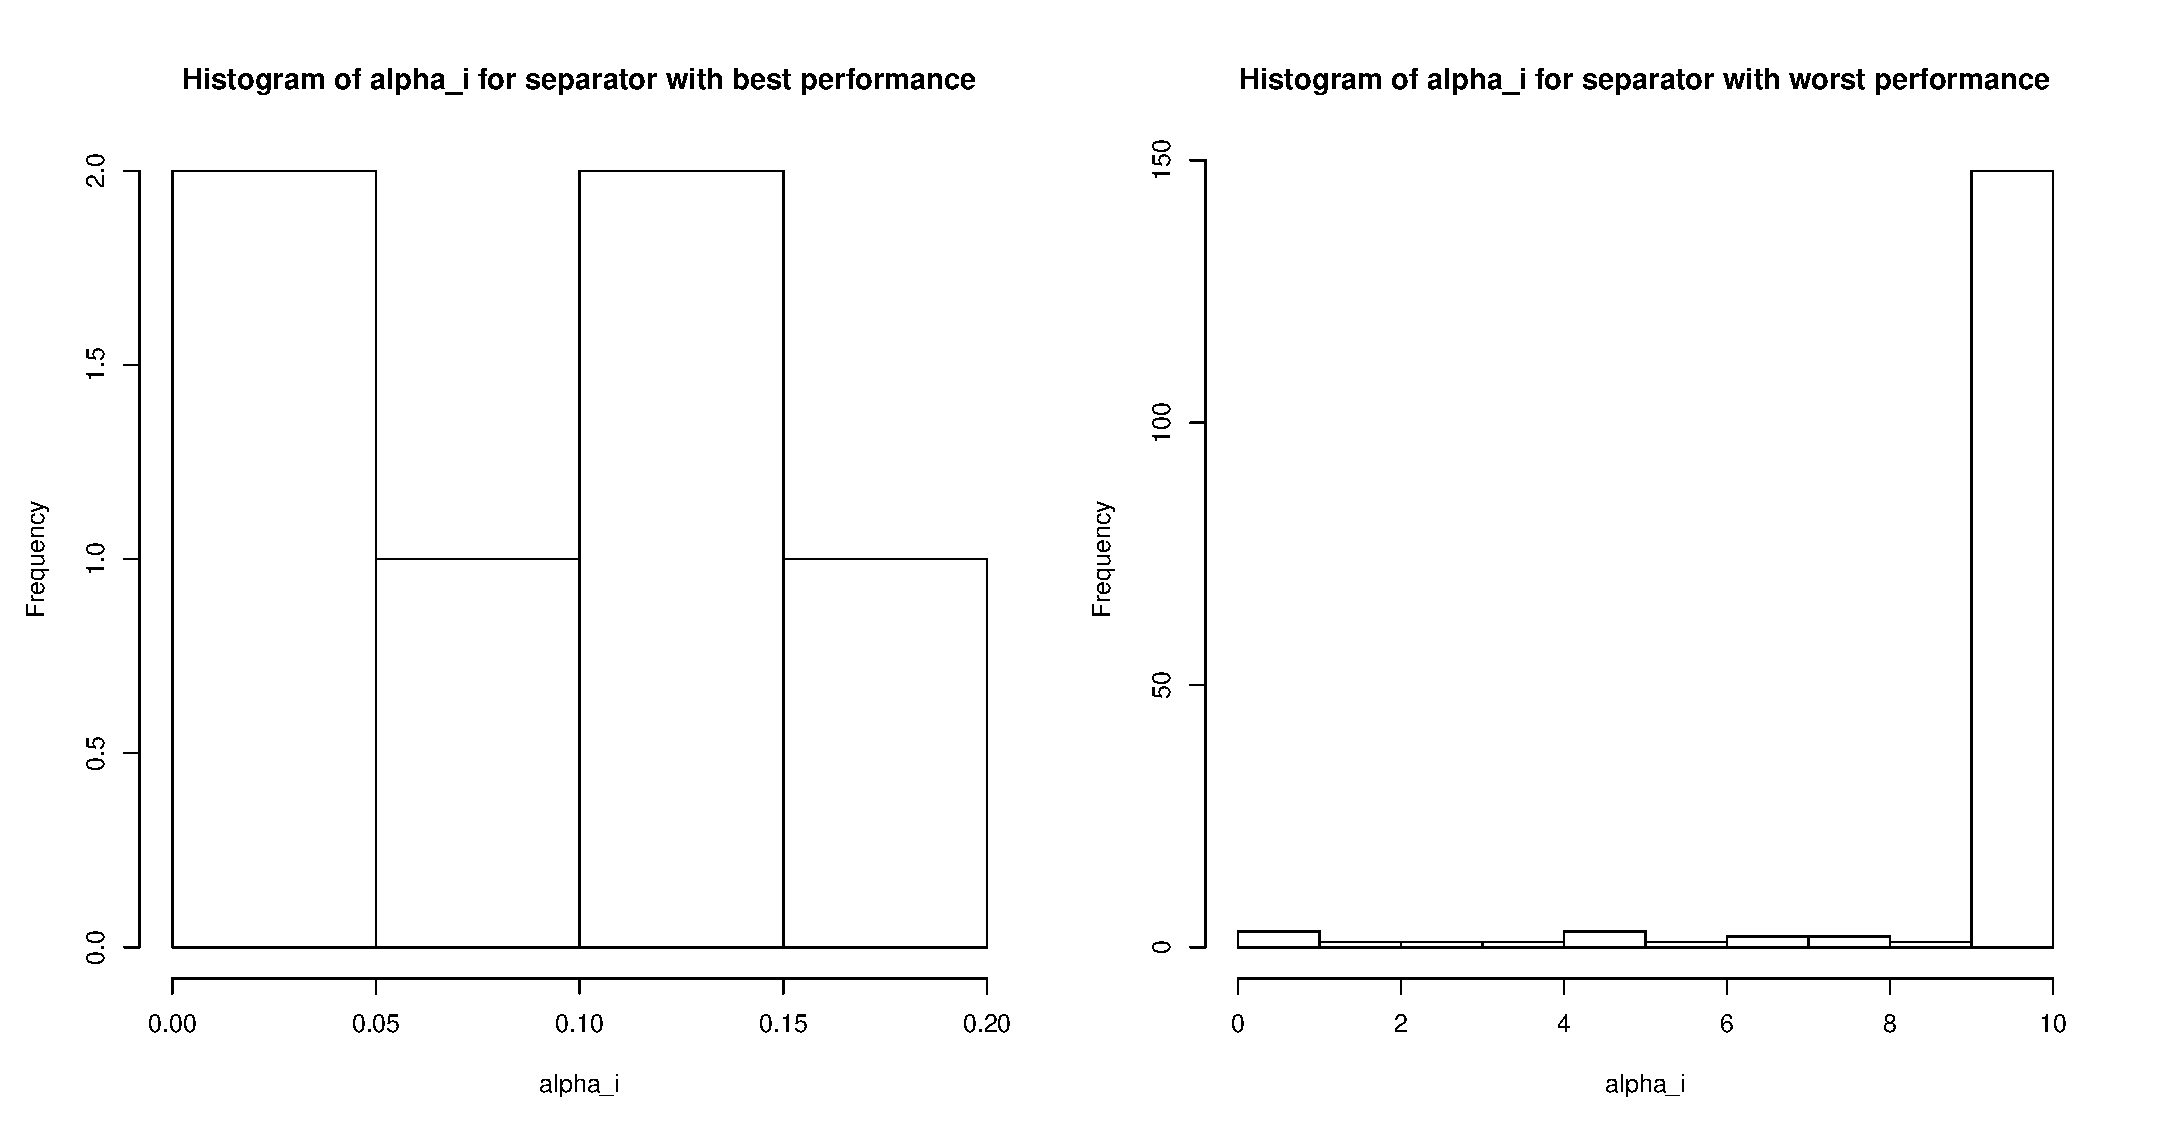
\includegraphics[width=12.1cm]{small_hist_linear.eps}
\caption{\textit{Histograms of $\alpha_{i}$ for SVM separators with best and worst performances by using linear kernel on small data set with optimal parameter. Left: best, separator over class 'foliage' and class 'sky', $\#$ of SVs is 6. Right: worst, separator over class 'foliage' and 'window', $\#$ of SVs is 163.}}
\end{figure}

%%% ------------------------------------------------------------------------------
\goodbreak

\newpage

\subsection{Polynomial Kernel}

The following table shows the accuracies by choosing different $c$ and $r$:

\scalebox{0.85}{
 \begin{tabular}{|c|c|c|c|c|c|c|}
  \hline
  \diagbox{r}{c} & 0.5           &    0.9        & 1             & 1.2           & 5             & 10            \\ \hline
  2              & $96.79654 \%$ & $97.22944 \%$ & $97.18615 \%$ & $97.31602 \%$ & $96.83983 \%$ & $96.79654 \%$ \\ \hline
  3              & $96.58009 \%$ & $96.58009 \%$ & $96.62338 \%$ & $96.58009 \%$ & $96.45022 \%$ & $96.36364 \%$ \\ \hline
  4              & $96.58009 \%$ & $96.58009 \%$ & $96.58009 \%$ & $96.53680 \%$ & $96.36364 \%$ & $96.36364 \%$ \\ \hline
  5              & $96.40693 \%$ & $96.40693 \%$ & $96.40693 \%$ & $96.40693 \%$ & $96.40693 \%$ & $96.40693 \%$ \\ \hline
 \end{tabular}
}

Next table shows the total number of supported vectors for different $c$ and $r$:

\scalebox{1}{
 \begin{tabular}{|c|c|c|c|c|c|c|}
  \hline
  \diagbox{r}{c} & 0.5 & 0.9 & 1   & 1.2 & 5   & 10  \\ \hline
  2              & 356 & 339 & 342 & 338 & 324 & 330 \\ \hline
  3              & 321 & 321 & 318 & 320 & 314 & 313 \\ \hline
  4              & 351 & 352 & 349 & 354 & 351 & 351 \\ \hline
  5              & 328 & 328 & 328 & 328 & 328 & 328 \\ \hline
 \end{tabular}
}

Therefore, we choose $c=1.2$ and $r=2$ as our optimal parameters. The following two tables shows the perfomance of the classifier by choosing optimal parameters. Figure 9 shows the supported vectors among all vectors. We can observe from these two tables that among the 21 SVM separators, separator over class 'brickface' and class 'path' has best perfomance, and separator over class 'foliage' and class 'window' has worst performance. Figure 10 shows the histogram of non-zero $\alpha_{i}$ for these two separators. 

\scalebox{0.82}{
 \begin{tabular}{|c|c|c|c|c|c|c|c|}
  \hline
  class     & brickface & cement    & foliage   & grass     & path      & sky       & window    \\ \hline
  brickface & NA        & $99.09\%$ & $100.0\%$ & $100.0\%$ & $100.0\%$ & $99.85\%$ & $99.09\%$ \\ \hline
  cement    & $1.46378$ & NA        & $97.88\%$ & $99.70\%$ & $100.0\%$ & $99.55\%$ & $95.91\%$ \\ \hline
  foliage   & $0.00000$ & $1.77847$ & NA        & $99.85\%$ & $100.0\%$ & $100.0\%$ & $93.94\%$ \\ \hline
  grass     & $0.00000$ & $0.63884$ & $0.47913$ & NA        & $99.85\%$ & $99.70\%$ & $99.70\%$ \\ \hline
  path      & $0.00000$ & $0.00000$ & $0.00000$ & $0.47913$ & NA        & $99.85\%$ & $100.0\%$ \\ \hline
  sky       & $0.47913$ & $1.02265$ & $0.00000$ & $0.63884$ & $0.47913$ & NA        & $99.85\%$ \\ \hline
  window    & $1.05940$ & $2.02651$ & $1.74955$ & $0.63884$ & $0.00000$ & $0.47913$ & NA        \\ \hline
 \end{tabular}
}

\scalebox{0.82}{
 \begin{tabular}{|c|c|c|c|c|c|c|c|}
  \hline
  class     & brickface & cement    & foliage   & grass     & path      & sky       & window    \\ \hline
  brickface & NA & 33 & 34 & 50 & 23 & 42 & 35 \\ \hline
  cement    & NA & NA & 39 & 39 & 50 & 30 & 69 \\ \hline
  foliage   & NA & NA & NA & 31 & 30 & 28 & 93 \\ \hline
  grass     & NA & NA & NA & NA & 40 & 41 & 38 \\ \hline
  path      & NA & NA & NA & NA & NA & 26 & 38 \\ \hline
  sky       & NA & NA & NA & NA & NA & NA & 32 \\ \hline
  window    & NA & NA & NA & NA & NA & NA & NA \\ \hline
 \end{tabular}
}

\begin{figure}[htp]
\centering
\includegraphics[width=12.1cm]{small_svm_polynomial.eps}
\caption{\textit{Projection of data into first two PC space. Here, ``cross'' represent the supported vector by using polynomial kernel, and the colors represent different classes: red--brickface, brown--sky, blue--foliage, green--cement, orange--window, grey--path, black--grass.}}
\end{figure}

\begin{figure}[htp]
\centering
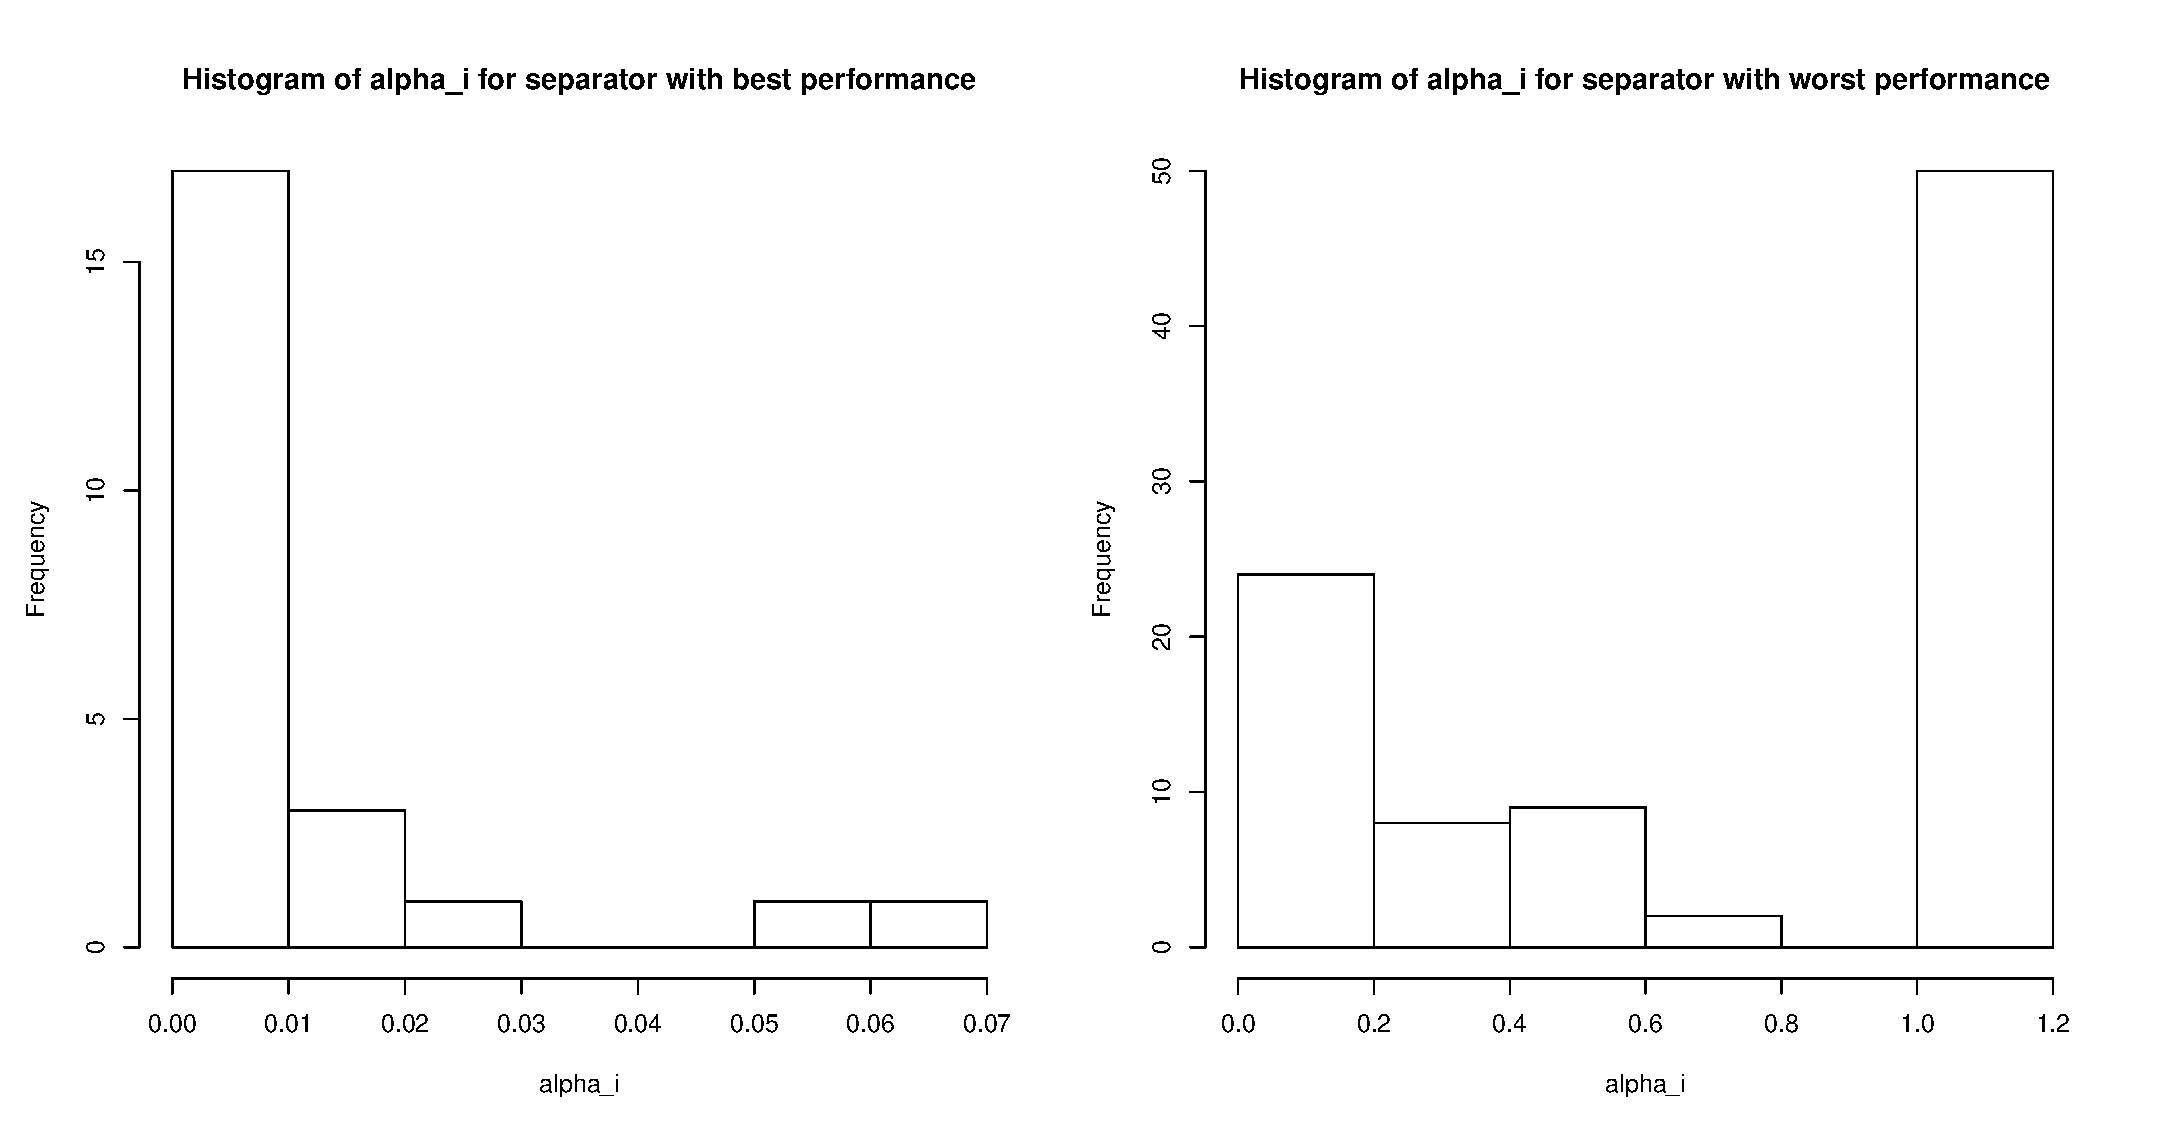
\includegraphics[width=12.1cm]{small_hist_polynomial.eps}
\caption{\textit{Histograms of $\alpha_{i}$ for SVM separators with best and worst performances by using polynomial kernel on small data set with optimal parameter. Left: best, separator over class 'brickface' and class 'path', $\#$ of SVs is 23. Right: worst, separator over class 'foliage' and 'window', $\#$ of SVs is 93.}}
\end{figure}

%%% ------------------------------------------------------------------------------
\goodbreak

\subsection{Gaussian Kernel}

At last, we will see the SVM by using Gaussian kernel, here, the parameters are $c$ and $\sigma$, in order to simplify the notation, we will use $\sigma^{*} = \frac{1}{2\sigma^{2}}$ in the following accuracy table:

\scalebox{0.82}{
 \begin{tabular}{|c|c|c|c|c|c|c|}
  \hline
  \diagbox{$\sigma^{*}$}{c} & 0.5           & 1             & 5             & 10            & 20            & 50            \\ \hline
  0.08                    & $93.50649 \%$ & $94.45887 \%$ & $96.36364 \%$ & $96.79654 \%$ & $96.79654 \%$ & $96.96970 \%$ \\ \hline
  0.1                     & $93.80952 \%$ & $94.63203 \%$ & $96.49351 \%$ & $96.92641 \%$ & $97.27273 \%$ & $97.09957 \%$ \\ \hline
  0.2                     & $93.67965 \%$ & $94.97835 \%$ & $96.75325 \%$ & $96.75325 \%$ & $96.92641 \%$ & $96.92641 \%$ \\ \hline
  0.4                     & $93.37662 \%$ & $95.45455 \%$ & $96.40693 \%$ & $96.40693 \%$ & $96.32035 \%$ & $96.36364 \%$ \\ \hline
  0.6                     & $93.11688 \%$ & $94.80519 \%$ & $95.49784 \%$ & $95.62771 \%$ & $95.71429 \%$ & $95.71429 \%$ \\ \hline
  0.8                     & $92.98701 \%$ & $94.45887 \%$ & $95.28139 \%$ & $95.41126 \%$ & $95.41126 \%$ & $95.36797 \%$ \\ \hline
  1                       & $92.51082 \%$ & $94.19913 \%$ & $94.97835 \%$ & $94.93506 \%$ & $94.89177 \%$ & $95.02165 \%$ \\ \hline
 \end{tabular}
}

Therefore, we choose $\sigma^{*}=0.1$ and $c=20$ as our optimal parameters. The following two tables shows the perfomance of the classifier by choosing optimal parameters. Figure 11 shows the supported vectors among all vectors. We can observe from these two tables that among the 21 SVM separators, separator over class 'brickface' and class 'path' has best perfomance, and separator over class 'foliage' and class 'window' has worst performance. Figure 12 shows the histogram of non-zero $\alpha_{i}$ for these two separators. 

\scalebox{0.82}{
 \begin{tabular}{|c|c|c|c|c|c|c|c|}
  \hline
  class     & brickface & cement    & foliage   & grass     & path      & sky       & window    \\ \hline
  brickface & NA        & $99.40\%$ & $99.85\%$ & $99.85\%$ & $100.0\%$ & $99.39\%$ & $99.85\%$ \\ \hline
  cement    & $1.05940$ & NA        & $99.09\%$ & $99.24\%$ & $100.0\%$ & $99.85\%$ & $95.45\%$ \\ \hline
  foliage   & $0.47913$ & $1.27769$ & NA        & $99.70\%$ & $100.0\%$ & $99.85\%$ & $95.00\%$ \\ \hline
  grass     & $0.47913$ & $1.47246$ & $0.63884$ & NA        & $99.70\%$ & $99.40\%$ & $99.55\%$ \\ \hline
  path      & $0.00000$ & $0.00000$ & $0.00000$ & $0.63884$ & NA        & $99.85\%$ & $100.0\%$ \\ \hline
  sky       & $1.05940$ & $0.47913$ & $0.47913$ & $1.05940$ & $0.47913$ & NA        & $99.70\%$ \\ \hline
  window    & $0.47913$ & $2.85700$ & $2.26429$ & $0.73189$ & $0.00000$ & $0.63884$ & NA        \\ \hline
 \end{tabular}
}

\scalebox{0.82}{
 \begin{tabular}{|c|c|c|c|c|c|c|c|}
  \hline
  class     & brickface & cement    & foliage   & grass     & path      & sky       & window    \\ \hline
  brickface & NA & 71 & 71 & 95 & 65 & 66 & 73 \\ \hline
  cement    & NA & NA & 95 & 87 & 112 & 83 & 112 \\ \hline
  foliage   & NA & NA & NA & 67 & 65 & 57 & 161 \\ \hline
  grass     & NA & NA & NA & NA & 85 & 62 & 83 \\ \hline
  path      & NA & NA & NA & NA & NA & 72 & 71 \\ \hline
  sky       & NA & NA & NA & NA & NA & NA & 58 \\ \hline
  window    & NA & NA & NA & NA & NA & NA & NA \\ \hline
 \end{tabular}
}

\begin{figure}[htp]
\centering
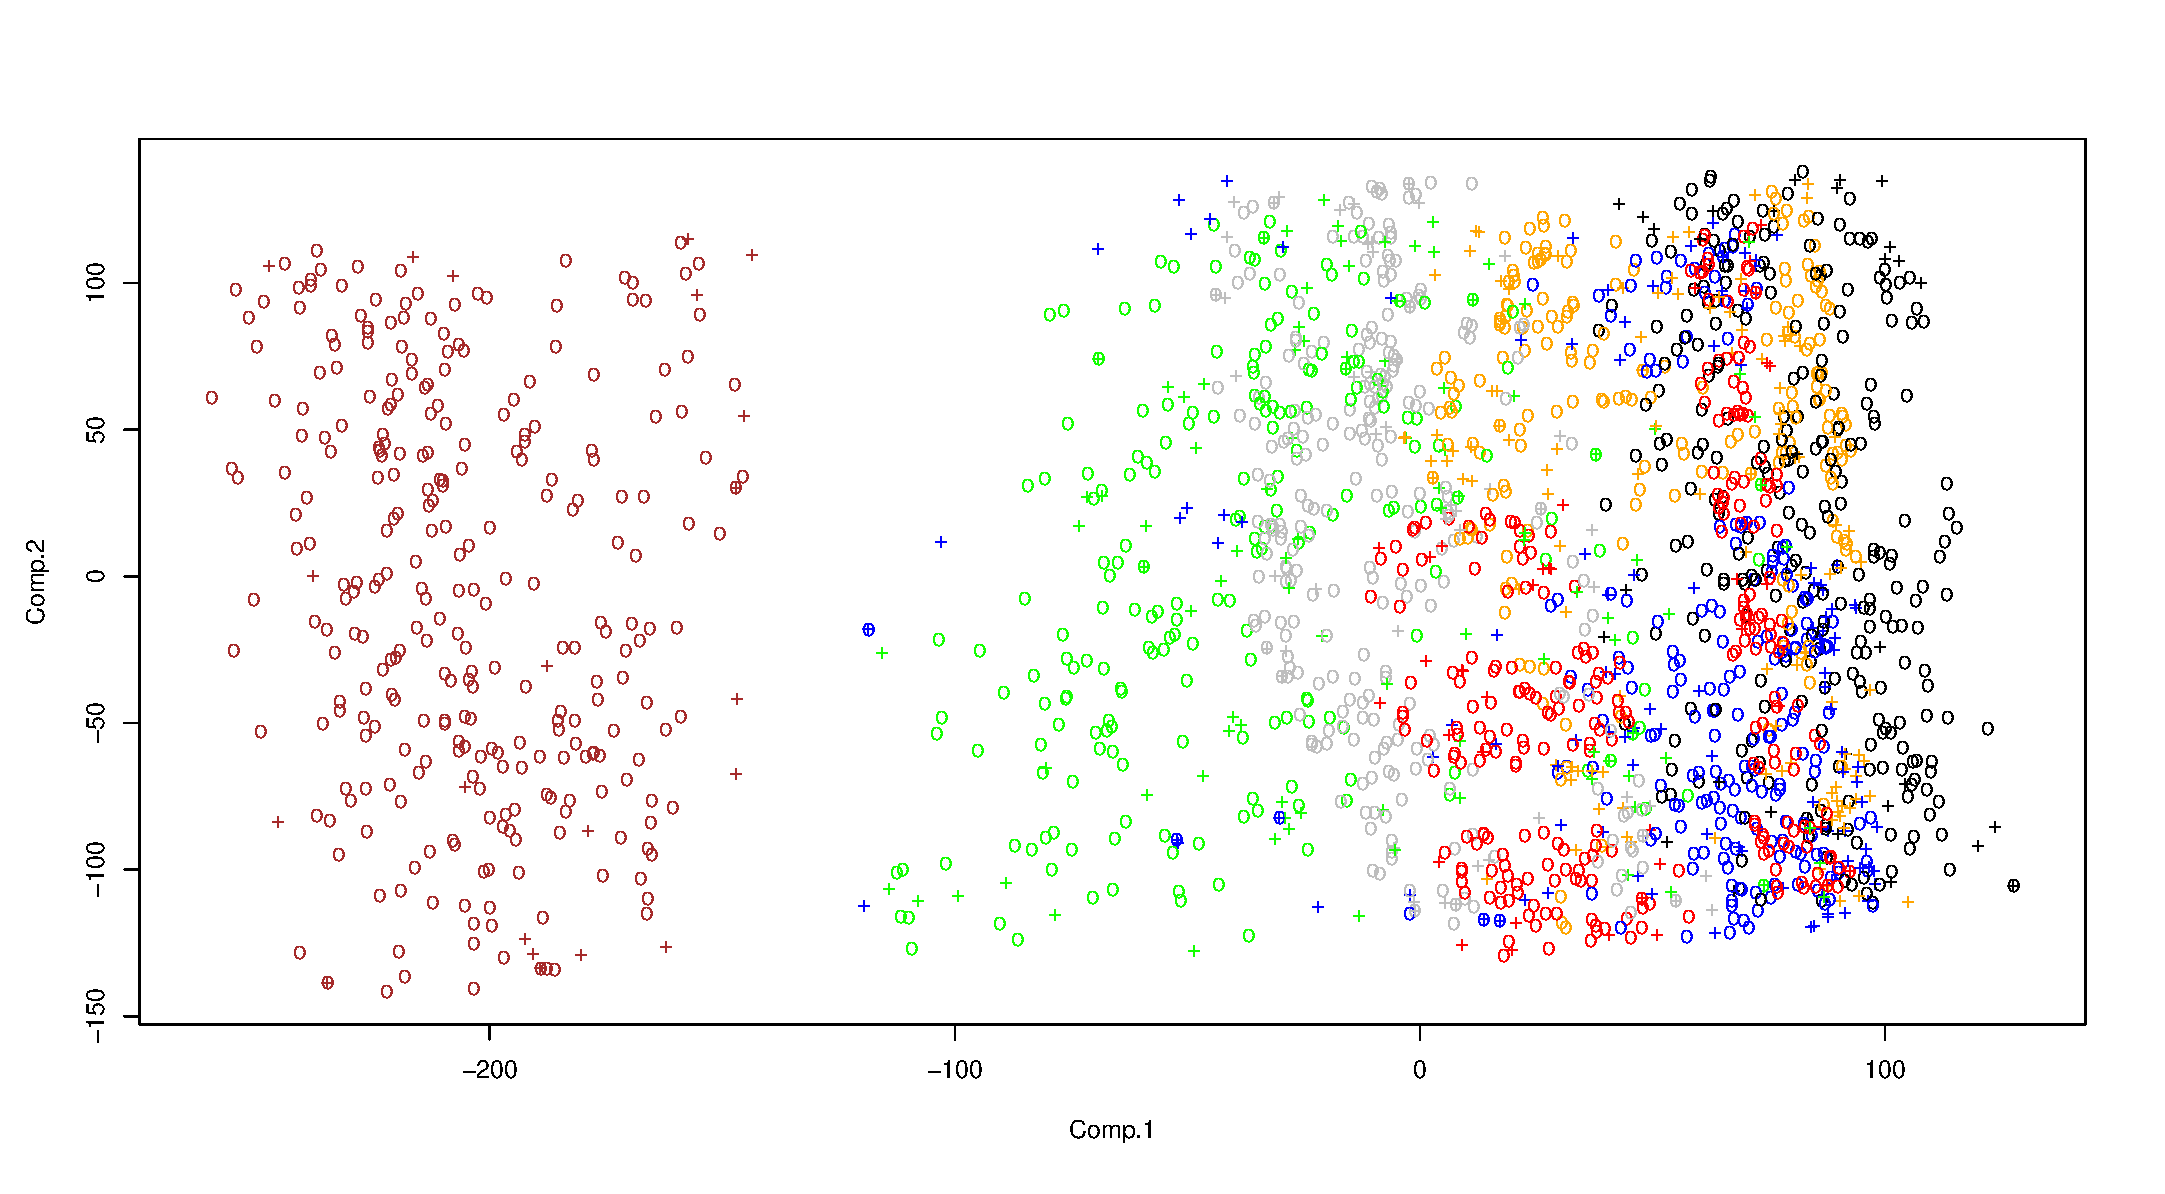
\includegraphics[width=12.1cm]{small_svm_gaussian.eps}
\caption{\textit{Projection of data into first two PC space. Here, ``cross'' represent the supported vector by using Gaussian kernel, and the colors represent different classes: red--brickface, brown--sky, blue--foliage, green--cement, orange--window, grey--path, black--grass.}}
\end{figure}

\begin{figure}[htp]
\centering
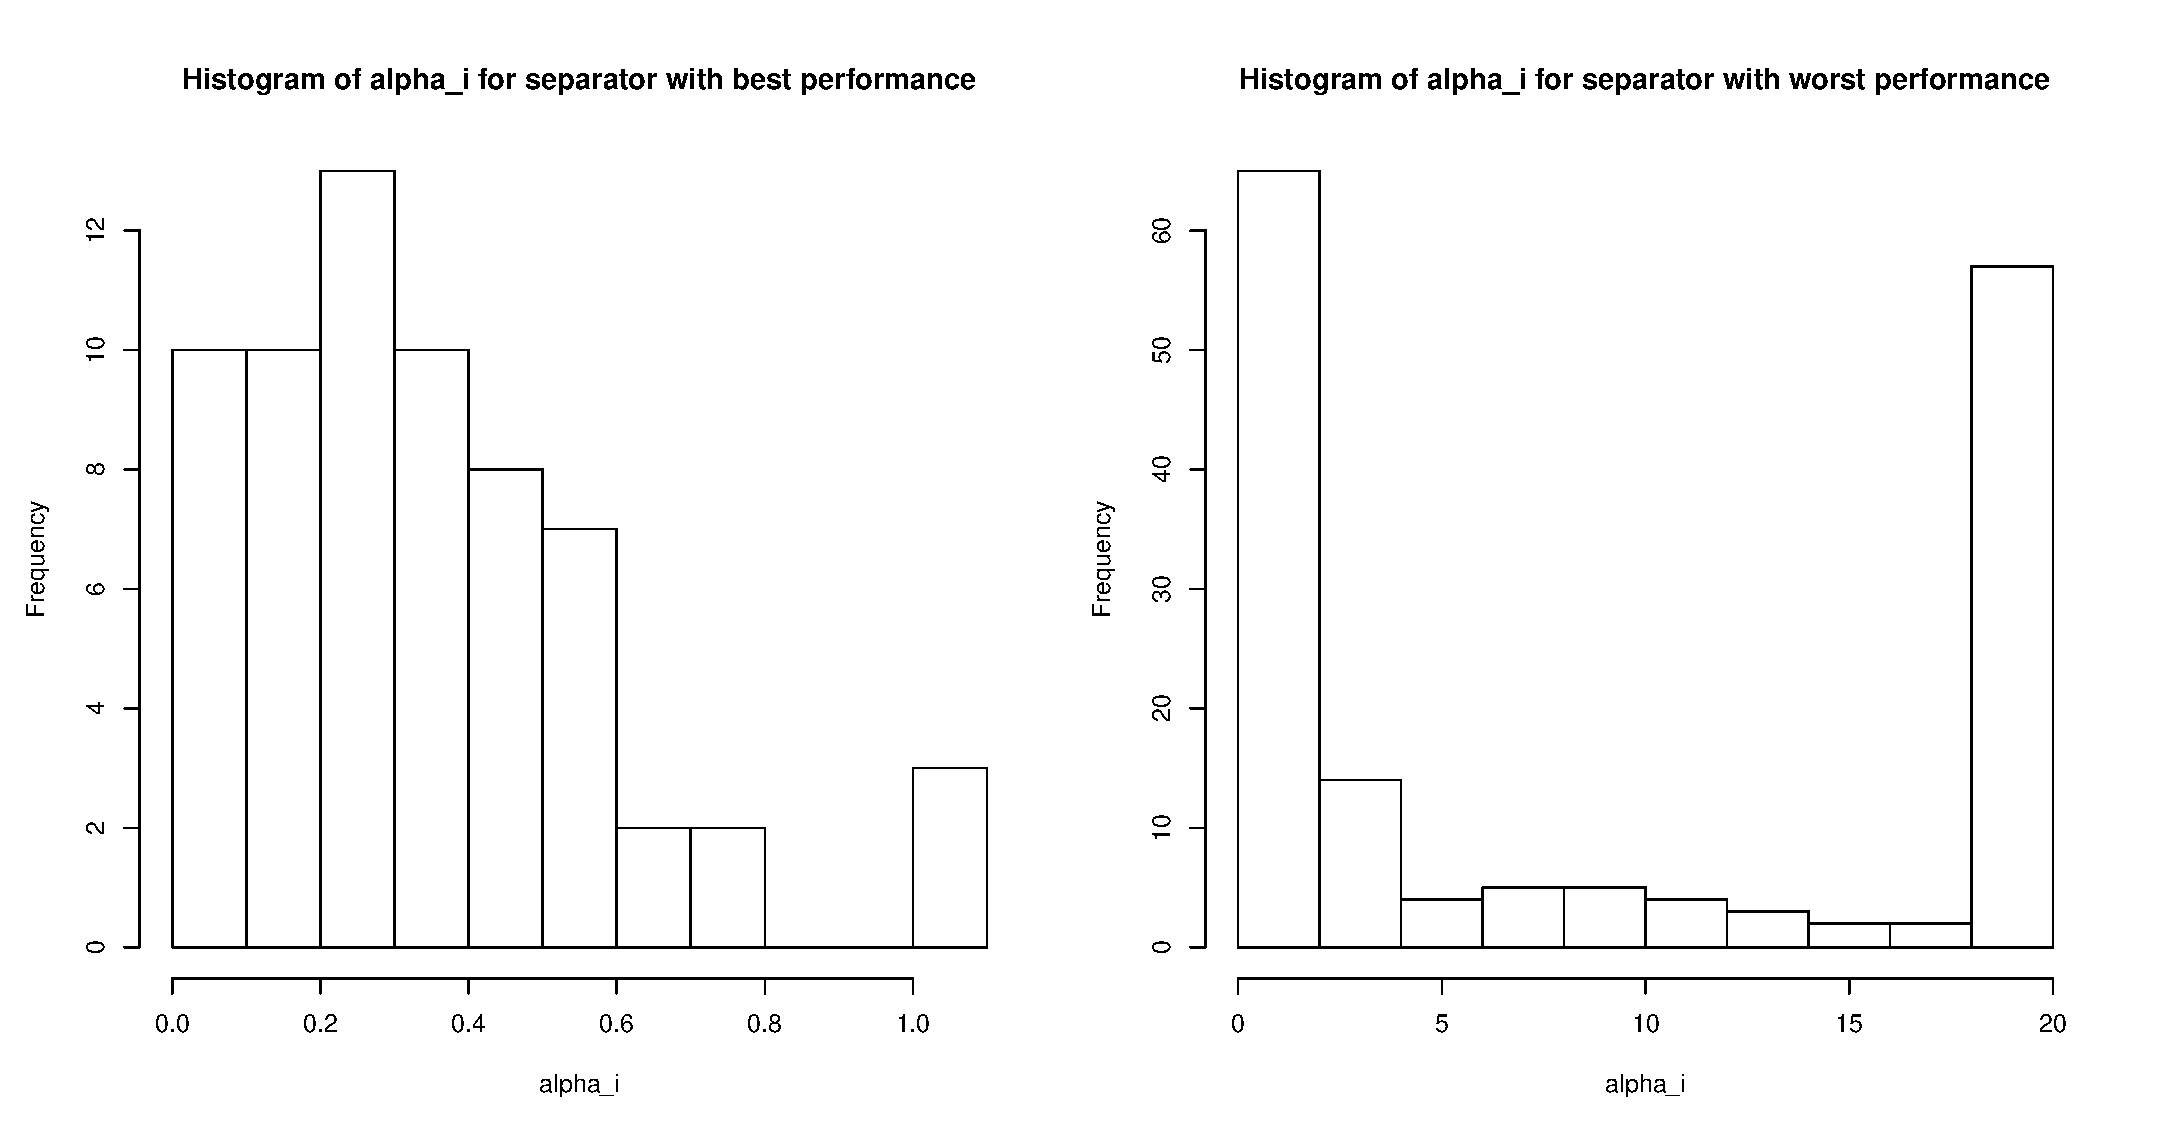
\includegraphics[width=12.1cm]{small_hist_gaussian.eps}
\caption{\textit{Histograms of $\alpha_{i}$ for SVM separators with best and worst performances by using Gaussian kernel on small data set with optimal parameter. Left: best, separator over class 'brickface' and class 'path', $\#$ of SVs is 65. Right: worst, separator over class 'foliage' and 'window', $\#$ of SVs is 161.}}
\end{figure}

%%% ------------------------------------------------------------------------------
\goodbreak

\newpage

\appendix

\section{Appendix: running times}

The following table shows the running time on large data sets (1593 observations, 256 descriptors, 10 classes):

\scalebox{1}{
 \begin{tabular}{|c|c|c|}
  \hline
  linear         & polynomial     & Gaussian       \\ \hline
  5.362499 secs & 14.70856 secs  & 9.907342 secs \\ \hline
 \end{tabular}
}

And the next table shows the running time on small data sets (2320 observations, 19 descriptors, 7 classes):

\scalebox{1}{
 \begin{tabular}{|c|c|c|}
  \hline
  linear         & polynomial     & Gaussian       \\ \hline
  0.7461352 secs & 0.685853 secs  & 0.8766298 secs \\ \hline
 \end{tabular}
}

\end{document}


